\section{Design}
FlashEigen is an external-memory eigensolver optimized for any fast I/O devices
such as a large SSD array to compute eigenvalues of sparse graphs. It takes
advantage of the flexible programming interface of the Anasazi framework and
focuses on optimizing sparse matrix sparse matrix multiplication and dense
matrix operations on SSDs.

\subsection{Eigensolver algorithm}

%\begin{figure}
%\centering
%\includegraphics[scale=0.35]{./SpMM.pdf}
%\vspace{-5pt}
%\caption{}
%\vspace{-5pt}
%\label{SpMM}
%\end{figure}

\begin{algorithm}
	\begin{algorithmic}[1]
		\For{i = 0, 1, ..., until convergence}
		\State (1) Update the subspace $S \in \mathbb{R}^{n \times m}$,
		\State (2) Solve the projected eigenproblem $S^TASy = S^TSy\theta$.
		\State (3) Compute the residual: $r = Kx - x\theta$, where
		\State\hspace{\algorithmicindent} $x = Sy$ (Ritz vector), $\theta = \rho(x)$ (Ritz value).
		\State (4) Test the convergence of a Ritz pair $(x, \rho(x))$.
		\EndFor
	\end{algorithmic}
	\caption{Pseudo code of a generic eigenvalue algorithm that compute eigenvalues
	of a square matrix $A$ with $n$ rows and columns.}
	\label{eigencode}
\end{algorithm}

The state-of-art eigenvalue algorithms compute eigenvalues with iterative
methods. Figure \ref{eigencode} shows the steps in an iteration.
Step (1) constructs a vector subspace $S \in \mathbb{R}^{n \times m}$, where
$n$ is the number of rows or columns of a sparse matrix and $m$ is the number
of vectors in the subspace. When computing eigenvalues of a sparse graph,
two key operations in this step are sparse matrix multiplication to construct
the subspace and reorthogonalization to fix float-point rounding errors.
A block extenion of an eigensolver updates multiple vectors in the subspace
in a single step, which leads to sparse matrix dense matrix multiplication.

\subsection{Sparse matrix multiplication} \label{spmm}
Sparse matrix multiplication is a computationally expensive
operation in an eigensolver due to random memory access. Sparse matrix vector
multiplication (SpMV) is usually limited by the random memory performance of
DRAM. Sparse matrix dense matrix multiplication (SpMM) increases data locality
and improve overall performance of an eigensolver. Therefore, a block extension
of an eigensolver is preferred.

To handle a sparse graph with billions of vertices, we perform sparse matrix
multiplication in semi-external memory (SEM),
i.e., the input and output vectors or dense matrices in memory and the sparse
matrix on SSDs. This strategy enables nearly in-memory performance while achieving
the scalability in proportion to the ratio of edges to vertices in a graph.

\subsubsection{The sparse matrix format}
The state-of-art numeric libraries store a sparse matrix in compressed row storage
(CSR) or compressed column storage (CSC) format. However, these formats incur
many CPU cache misses in sparse matrix multiplication on many real-world graphs
due to their nearly random vertex connection. They also require a relatively
large storage size. For a graph with billions of edges, we have to use eight
bytes to store the row and column indices. For semi-external memory sparse
matrix multiplication, a large matrix format may cause SSDs to be the bottleneck.
Therefore, we need to use an alternative format for sparse matrices to increase
CPU cache hits and reduce the amount of data read from SSDs.

\begin{figure}
\centering
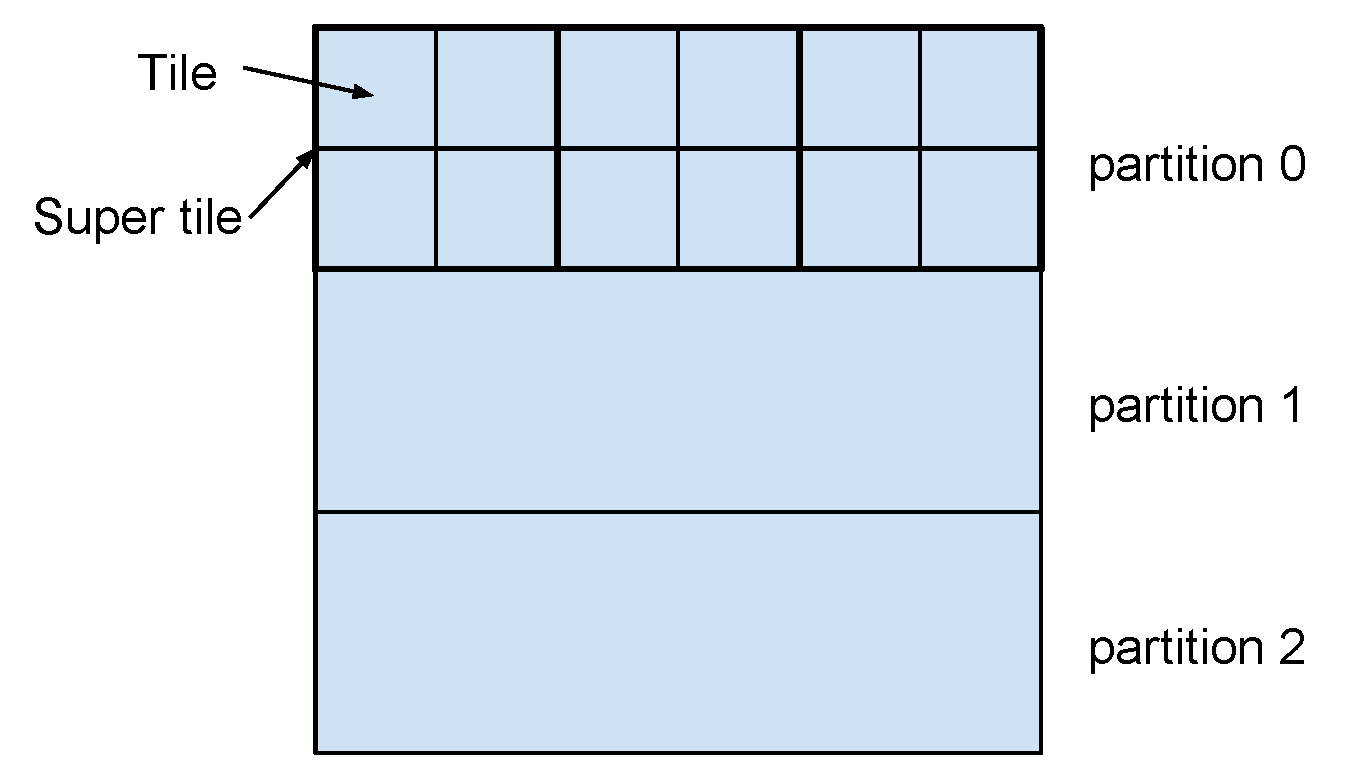
\includegraphics[scale=0.3]{./sparse_mat.pdf}
\vspace{-5pt}
\caption{}
\vspace{-5pt}
\label{sparse_mat}
\end{figure}

To increase CPU cache hits, we deploy cache blocking \cite{Im04} and store
non-zero entries in a sparse matrix in tiles (Figure \ref{sparse_mat}).
When a tile is small, the rows of the input and output dense matrices
involved in the multiplication with the tile are always kept in the CPU cache
during the multiplication. The optimal tile size should fill the CPU cache
with the rows of the dense matrices involved in the multiplication with
the tile and is affected by the number of columns of the dense matrices.
The number of columns of these dense matrices are chosen by users. Instead
of generating a sparse matrix with
different tile sizes optimized for different numbers of columns in the dense
matrices, we use a relatively small tile size and rely on the runtime system
to optimize for different numbers of columns (in section \ref{sec:exec}).
In the semi-external memory mode, we expect that the dense matrices do not
have more than eight columns in sparse matrix multiplication. By default, we
use the tile size of $16K \times 16K$ to the matrix storage size and
the adaptibility to different numbers of columns.

\begin{figure}
\centering
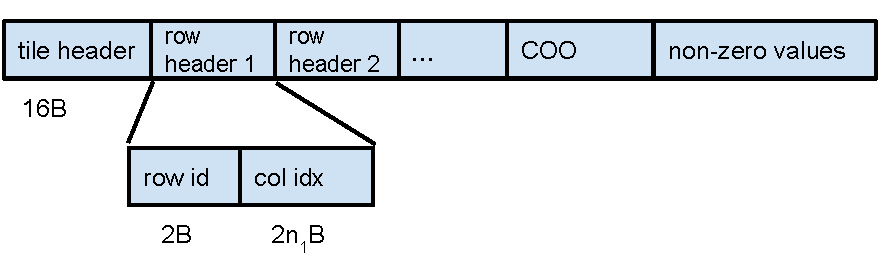
\includegraphics[scale=0.5]{./tile_format.pdf}
\vspace{-5pt}
\caption{The storage format of a tile in a sparse matrix.}
\vspace{-5pt}
\label{tile_format}
\end{figure}

To reduce the overall storage size of a sparse matrix, we use a compact format
to store non-zero entries in a tile. In very sparse matrices such as
many real-world graphs, many rows in a tile do not have any non-zero entries.
The CSR (CSC) format requires an entry for each row (column) in the row
(column) index. Therefore, the CSR or CSC format waste space when storing elements
in a tile. Instead, we only keeps data for rows with non-zero entries in a tile
shown in Figure \ref{tile_format}. For rows with more than one non-zero entries,
we use a variant of the CSR format, which maintains a row header for each row.
A row header has an identifier to indicate the row number, followed by column
indices. We refer to this format as SCSR (Super Compressed Row Storage).
The most significant bit of the identifier is always set to 1, while the most
significant bit of a column index entry is always set to 0. As such, we can easily
distinguish a row identifier from a column index entry and determine the end
of a row. Thanks to the small size of a tile, we use two bytes to store a row
number and a column index entry to reduce the storage size. Since the most
significant bit is used to indicate the beginning of a row, the maximum tile size
is $32K \times 32K$.

For many real-world graphs, many rows in a tile have only one non-zero entries,
thanks to their nearly random vertex connection. Storing these single-entry
rows in separate rows results in many conditional jump CPU instructions in
sparse matrix multiplication.
In contrast, the coordinate format (COO) is more suitable for storing these
single-entry rows. It does not increase the storage size but significantly
reduces the number of conditional jump instructions when we iterate
them. As a result, we hybrid SCSR and COO to store non-zero entries in a tile
with COO stored behind the row headers of SCSR. All non-zero entries are
stored together at the end of a tile.

We organize tiles in a sparse matrix in tile rows and maintain a matrix index
for them. Each entry of the index stores the location of a tile row on SSDs
to facilitate random access
to tile rows. This is useful for parallelizing sparse matrix multiplication.
Because a tile contains thousands of rows, the matrix index requires a very
small storage size even for a billion-node graph. We keep the entire index
in memory during sparse matrix multiplication.

\subsubsection{The dense matrix format for SpMM} \label{numa_mat}
The dense matrix in sparse matrix multiplication is a tall-and-skinny matrix
with millions or even billions of rows but only several columns. For sparse
matrix multiplication, we organize elements of the dense matrix in row-major
order to increase data locallity, as shown in Figure \ref{dense_mat} (a).

For a non-uniform memory architecture (NUMA), we partition the input dense matrix
horizontally and store partitions evenly across NUMA nodes to fully utilize
the bandwidth of memory and inter-processor links in sparse matrix
multiplication. The NUMA architecture is commonly used in today's multi-processor
servers, where each processor connects to its own memory banks. It is essential
to fully utilize the bandwidth of memory and inter-processor links to achieve
performance. As shown in Figure \ref{dense_mat} (a), we assign multiple
contiguous rows to a partition and assign multiple partitions to the same
NUMA node. A partition always has $2^i$ rows for efficiently locating a row
with bit operations. The partition size is also multiple of the tile size of
a sparse matrix so that multiplication on a tile only needs to access rows
from a single partition.

\begin{figure}
\centering
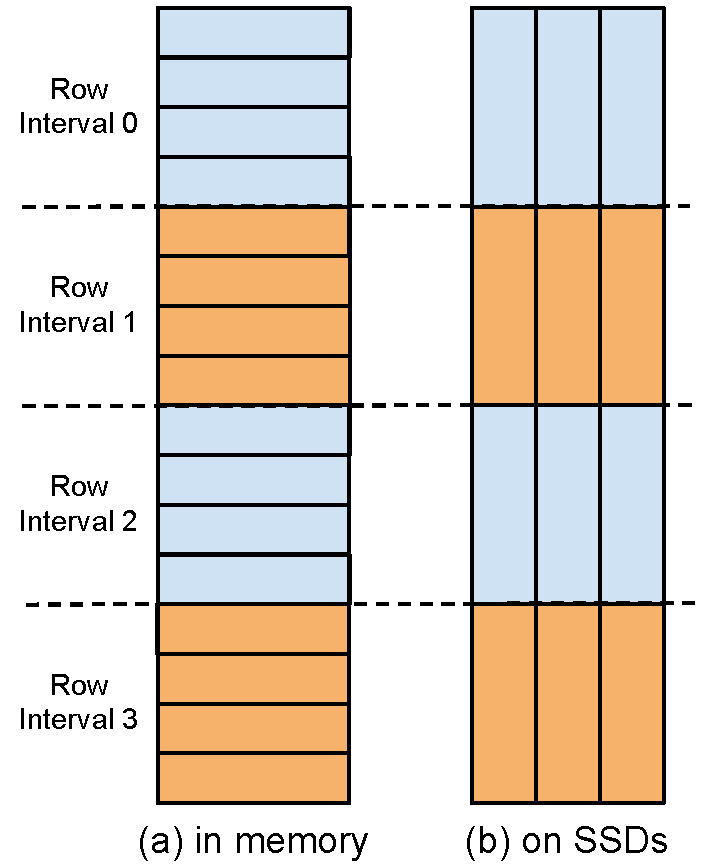
\includegraphics[scale=0.4]{./dense_matrix.pdf}
\vspace{-5pt}
\caption{The data layout of tall-and-skinny dense matrices. A tall-and-skinny
dense matrix is partitioned horizontally into many row intervals.
(a) For an in-memory matrix, row intervals are stored across NUMA nodes and
elements are stored in row-major order; (b) for an SSD-based matrix, elements
inside a partition are stored in column-major order.}
\vspace{-5pt}
\label{dense_mat}
\end{figure}

\subsubsection{Execution of sparse matrix multiplication} \label{sec:exec}
We perform sparse matrix dense matrix in semi-external memory.
We optimize sparse matrix dense matrix multiplication at runtime for different
numbers of columns in the dense matrices.

We partition a sparse matrix horizontally for parallelization and assign multiple
contiguous tile rows to the same partition (Figure \ref{sparse_mat}).
The number of tile rows assigned to a partition is determined at runtime by
the number of columns in the input dense matrix.
\dz{Can we just give a fixed number of tile rows to a partition and use
the hilbert curve to process tiles?}
A thread reads a partition of the sparse matrix
asynchronously from SSDs. Once a partition is ready in memory, the worker
thread multiplies the partition with the input dense matrix, which generates
a portion of the output matrix. To reduce memory consumption,
we write the portion of the output dense matrix to SSDs immediately whenever
it is generated.
\dz{Implement this.}

To better utilize CPU cache, we process tiles of a partition in
\textit{super tile}s (Figure \ref{sparse_mat}). The tile size of a sparse
matrix is specified when the sparse matrix image is created and is relatively
small to handle different numbers of columns in the dense matrices.
A \textit{super tile} is composed of tiles from multiple tile rows and its
size is determined at runtime by three factors: the number of columns
in the dense matrices, the CPU cache size and the number of threads that
share the CPU cache. An optimal size for a \textit{super tile} fills
the CPU cache with the rows from the dense matrices involved in
the computation with the \textit{super tile}.
\dz{Should I give an example here?}

Load balancing also plays a key role in sparse matrix multiplication on
many real-world graphs due to their power-law distribution in vertex degree.
In FlashEigen, a worker thread first processes partitions with more non-zero
entries, originally assigned to the thread. When a worker thread finishes
all of its own partitions, it steals partitions that have not been processed
from other worker threads.

In spite of nearly random distribution of non-zero entries in a sparse matrix,
there exists regularity that allows vectorization to improve performance
in sparse matrix dense matrix multiplication. For each non-zero entry, we
need to multiply it with the corresponding row from the input dense matrix
and add the result to the corresponding row in the output dense matrix.
These operations can be accomplished by the vector CPU instructions such as
AVX \cite{avx}.

\subsection{Dense matrix operations}
The vector subspace maintained by an eigensolver is massive when the eigensolver
computes a few eigenvalues of a billion-node graph or computes many eigenvalues
of a multi-million-node graph. The number of vectors required for the subspace
increases as the number of required eigenvalues increases. Furthermore, a larger
number of vectors in the subspace improves the convergence rate of an eigensolver. 
It is often that an eigensolver needs multiple terabytes to store the vectors
in the subspace for these eigenvalue problems. Therefore, FlashEigen stores
vectors on SSDs.

FlashEigen stores multiple vectors of the subspace in a dense matrix physically.
One reason is that the Anasazi eigensolvers update multiple vectors of the subspace
in an iteration due to the block extension of the eigenvalue algorithms.
This design also helps garbage collection in lazy evaluation (section \ref{sec:lazy_eval}).
As such, the subspace is composed of tall-and-skinny dense
matrices. However, the eigensolvers still need to access individual vectors,
so we organize the elements in the dense matrices in column-major order. 
The Anasazi eigensolvers require the dense matrix operations shown in Figure
\ref{anasazi_ops}.
\begin{table}
	\begin{center}
		\small
		\begin{tabular}{|c|c|c|c|c|}
			\hline
			& operation & customized output \\
			\hline
			op1 & $CC \leftarrow \alpha \times AA \times B + \beta \times CC$ & yes \\
			\hline
			op2 & $BB \leftarrow AA \times diag(vec)$ & yes \\
			\hline
			op3 & $A \leftarrow \alpha \times t(AA) \times BB$ & no \\
			\hline
			op4 & $CC \leftarrow \alpha \times AA + \beta \times BB$ & yes \\
			\hline
			op5 & $BB \leftarrow \alpha \times AA$ & yes \\
			\hline
			op6 & $vec \leftarrow norm\_col(AA)$ & no \\
			\hline
			op7 & $BB \leftarrow AA[,idxs]$ & yes \\
			\hline
			op8 & $AA[,idxs] \leftarrow BB$ & yes \\
			\hline
		\end{tabular}
		\normalsize
	\end{center}
	\caption{The dense matrix operations required by the Anasazi eigensolvers.
		$XX$ represents a tall dense matrix, $X$ represents a small dense matrix,
	$\alpha$ and $\beta$ represents scalar variables.}
	\label{anasazi_ops}
\end{table}
The Anasazi eigensolvers allow users to implement the tall-and-skinny matrices
and their operations.

It is challenging to achieve the performance of external-memory dense matrix
operations comparable to their in-memory counterparts. Unlike sparse matrix
multiplication, these dense matrix operations are less \dz{computationally
expensive}. Even though SSDs are fast, their sequential I/O performance is
still an order of magnitude slower than RAM. Therefore, dense matrix operations
on SSDs are significantly slower than the ones in RAM (Figure \ref{perf:mat_ops}).
Furthermore, SSDs wears out after a certain amount of write \cite{}, so
even enterprise SSDs \cite{} only allows a small number of DWPD
(diskful writes per day). Therefore, FlashEigen optimizes dense matrix operations
with the following goals: \textit{(i)} reduce writes to SSDs, \textit{(ii)}
reduce reads from SSDs, \textit{(iii)} reduce computation.

\begin{figure}
	\begin{center}
		\footnotesize
		\vspace{-15pt}
		\begin{tikzpicture}[gnuplot]
%% generated with GNUPLOT 4.6p4 (Lua 5.1; terminal rev. 99, script rev. 100)
%% Thu 16 Jul 2015 09:41:54 AM EDT
\path (0.000,0.000) rectangle (8.382,4.572);
\gpcolor{color=gp lt color border}
\gpsetlinetype{gp lt border}
\gpsetlinewidth{1.00}
\draw[gp path] (1.320,0.616)--(1.500,0.616);
\draw[gp path] (7.829,0.616)--(7.649,0.616);
\node[gp node right] at (1.136,0.616) { 0};
\draw[gp path] (1.320,1.436)--(1.500,1.436);
\draw[gp path] (7.829,1.436)--(7.649,1.436);
\node[gp node right] at (1.136,1.436) { 5};
\draw[gp path] (1.320,2.256)--(1.500,2.256);
\draw[gp path] (7.829,2.256)--(7.649,2.256);
\node[gp node right] at (1.136,2.256) { 10};
\draw[gp path] (1.320,3.075)--(1.500,3.075);
\draw[gp path] (7.829,3.075)--(7.649,3.075);
\node[gp node right] at (1.136,3.075) { 15};
\draw[gp path] (1.320,3.895)--(1.500,3.895);
\draw[gp path] (7.829,3.895)--(7.649,3.895);
\node[gp node right] at (1.136,3.895) { 20};
\draw[gp path] (2.250,0.616)--(2.250,0.796);
\draw[gp path] (2.250,3.895)--(2.250,3.715);
\node[gp node center] at (2.250,0.308) {op1};
\draw[gp path] (3.180,0.616)--(3.180,0.796);
\draw[gp path] (3.180,3.895)--(3.180,3.715);
\node[gp node center] at (3.180,0.308) {op2};
\draw[gp path] (4.110,0.616)--(4.110,0.796);
\draw[gp path] (4.110,3.895)--(4.110,3.715);
\node[gp node center] at (4.110,0.308) {op3};
\draw[gp path] (5.039,0.616)--(5.039,0.796);
\draw[gp path] (5.039,3.895)--(5.039,3.715);
\node[gp node center] at (5.039,0.308) {op4};
\draw[gp path] (5.969,0.616)--(5.969,0.796);
\draw[gp path] (5.969,3.895)--(5.969,3.715);
\node[gp node center] at (5.969,0.308) {op5};
\draw[gp path] (6.899,0.616)--(6.899,0.796);
\draw[gp path] (6.899,3.895)--(6.899,3.715);
\node[gp node center] at (6.899,0.308) {op6};
\draw[gp path] (1.320,3.895)--(1.320,0.616)--(7.829,0.616)--(7.829,3.895)--cycle;
\node[gp node center,rotate=-270] at (0.246,2.255) {Ratio (in-mem/EM)};
\def\gpfillpath{(2.250,0.616)--(2.561,0.616)--(2.561,1.709)--(2.250,1.709)--cycle}
\gpfill{color=gpbgfillcolor} \gpfillpath;
\gpfill{color=gp lt color 0,gp pattern 0,pattern color=.} \gpfillpath;
\gpcolor{color=gp lt color 0}
\gpsetlinetype{gp lt plot 0}
\draw[gp path] (2.250,0.616)--(2.250,1.708)--(2.560,1.708)--(2.560,0.616)--cycle;
\def\gpfillpath{(3.180,0.616)--(3.491,0.616)--(3.491,3.193)--(3.180,3.193)--cycle}
\gpfill{color=gpbgfillcolor} \gpfillpath;
\gpfill{color=gp lt color 0,gp pattern 0,pattern color=.} \gpfillpath;
\draw[gp path] (3.180,0.616)--(3.180,3.192)--(3.490,3.192)--(3.490,0.616)--cycle;
\def\gpfillpath{(4.110,0.616)--(4.421,0.616)--(4.421,1.593)--(4.110,1.593)--cycle}
\gpfill{color=gpbgfillcolor} \gpfillpath;
\gpfill{color=gp lt color 0,gp pattern 0,pattern color=.} \gpfillpath;
\draw[gp path] (4.110,0.616)--(4.110,1.592)--(4.420,1.592)--(4.420,0.616)--cycle;
\def\gpfillpath{(5.039,0.616)--(5.350,0.616)--(5.350,3.555)--(5.039,3.555)--cycle}
\gpfill{color=gpbgfillcolor} \gpfillpath;
\gpfill{color=gp lt color 0,gp pattern 0,pattern color=.} \gpfillpath;
\draw[gp path] (5.039,0.616)--(5.039,3.554)--(5.349,3.554)--(5.349,0.616)--cycle;
\def\gpfillpath{(5.969,0.616)--(6.280,0.616)--(6.280,2.927)--(5.969,2.927)--cycle}
\gpfill{color=gpbgfillcolor} \gpfillpath;
\gpfill{color=gp lt color 0,gp pattern 0,pattern color=.} \gpfillpath;
\draw[gp path] (5.969,0.616)--(5.969,2.926)--(6.279,2.926)--(6.279,0.616)--cycle;
\def\gpfillpath{(6.899,0.616)--(7.210,0.616)--(7.210,2.152)--(6.899,2.152)--cycle}
\gpfill{color=gpbgfillcolor} \gpfillpath;
\gpfill{color=gp lt color 0,gp pattern 0,pattern color=.} \gpfillpath;
\draw[gp path] (6.899,0.616)--(6.899,2.151)--(7.209,2.151)--(7.209,0.616)--cycle;
\gpcolor{color=gp lt color border}
\gpsetlinetype{gp lt border}
\draw[gp path] (1.320,3.895)--(1.320,0.616)--(7.829,0.616)--(7.829,3.895)--cycle;
%% coordinates of the plot area
\gpdefrectangularnode{gp plot 1}{\pgfpoint{1.320cm}{0.616cm}}{\pgfpoint{7.829cm}{3.895cm}}
\end{tikzpicture}
%% gnuplot variables

		\vspace{-15pt}
		\caption{The relative performance of external-memory matrix operations
			on a dense matrix with 200M rows and 16 columns on an array of 24
		SSDs.}
		\label{perf:mat_ops}
	\end{center}
\end{figure}

\subsubsection{Parallelization and external memory access}
We partition the tall-and-skinny matrices horizontally for parallelization
and external-memory access. Figure \ref{dense_mat} (b) illustrates the format
of such a dense matrix. Like a NUMA dense matrix in Figure \ref{dense_mat} (a),
each partition contains multiple contiguous rows in a row interval and data
in a partition is stored contiguously. Unlike a NUMA dense matrix, elements
in a partition of a dense matrix on SSDs are stored in column-major order
for easily accessing individual columns. Each partition is roughly 4MB
\dz{what is the right size?} to balance memory consumption and I/O performance.
The size of a row interval is chosen according to the number of columns in
the matrix to meet the partition size.

Once data in a partition is loaded to memory, we further partition it to
smaller row intervals so that data
in the sub-row-interval fits in CPU cache. \dz{TODO: The size of the sub row
interval should also adapt to the matrix width.} This optimization is essential
for matrix multiplication because . so when we copy the data in
the sub row interval to a piece of contiguous memory, all data can be kept in
memory.

\begin{figure}
\centering
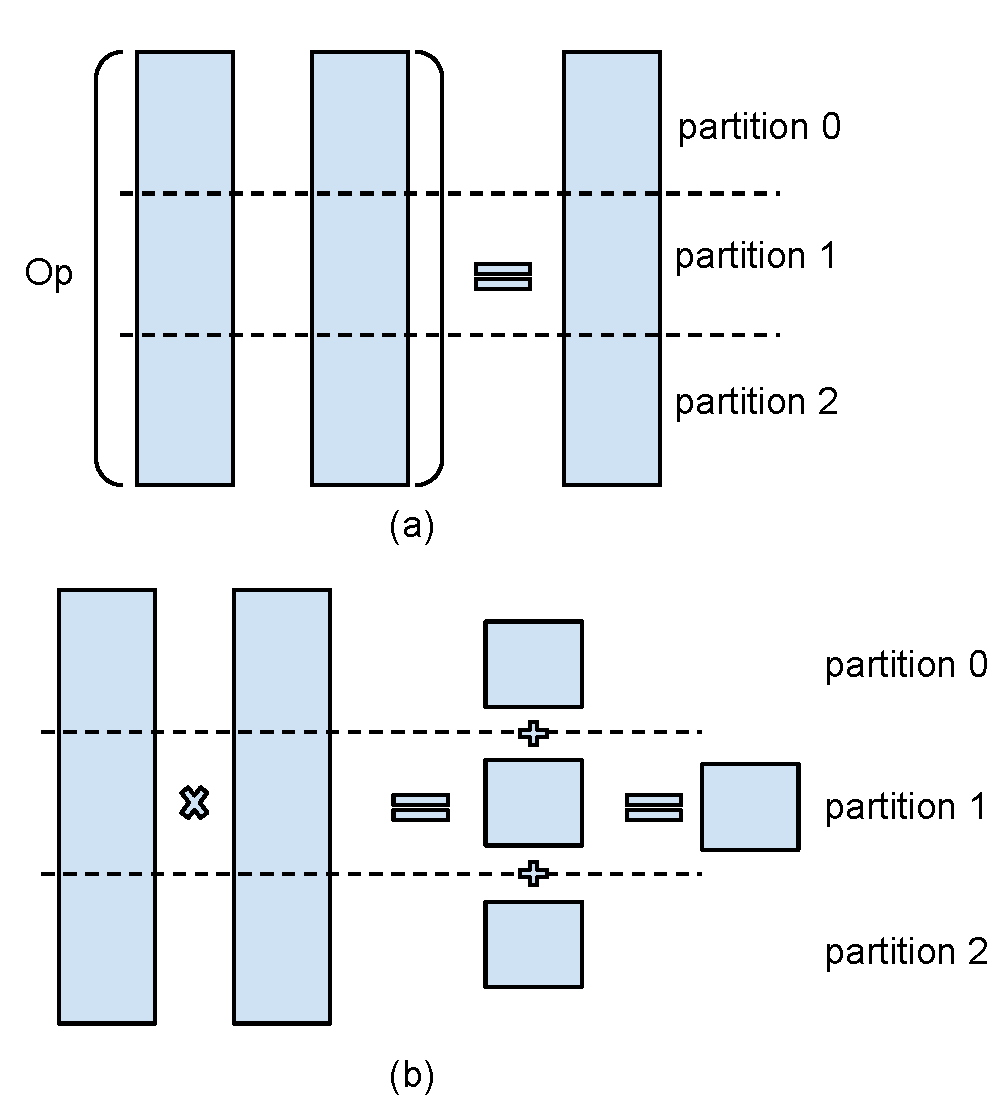
\includegraphics[scale=0.4]{./mat_par.pdf}
\vspace{-5pt}
\caption{}
\vspace{-5pt}
\label{fig:mat_par}
\end{figure}

We assign the partitions in the same row interval from all of the tall-and-skinny
matrices in an operation to the same thread for parallel processing.
%(Figure \ref{fig:mat_par}).
Majority of the operations in Table \ref{anasazi_ops} output tall-and-skinny
matricies whose rows only depend on the same rows of the input matrices.
For these operations, the computation and data access to the tall-and-skinny
matrices are completely independant between row intervals. 
In contrast, $op3$ outputs a small matrix, but this operation can be split into
two operations: the first operation performs computation on all partitions
in the same row interval from
the input matrices and output a small matrix; the second operation
sums all of the small matrices and outputs a single small matrix.
%This is illustrated in Figure \ref{fig:mat_par}.
$op6$ can be evaluated in a similar fashion to $op3$.
Therefore, all matrix operations in Table \ref{anasazi_ops} can be parallelized
in the same fashion.

We maintain a global work queue to dispatch row intervals to threads dynamically.
As such, we minimize load imbalancing. This strategy also allows worker threads
to process row intervals close to each other, which helps to accumulate very large
writes to SSDs.

\dz{a large write is required to achieve persistent write performance and
wearout?}

We access partitions of the tall-and-skinny matrices in a sequential order
when performing an operation. If the partitions of these matrices are mapped
to SSDs in the order, all I/O accesses may hit some of the SSDs and saturate
them while other SSDs do not get any I/O access. To avoid the skew of I/O access,
we stripe data of a matrix across SSDs with a different order to improve I/O
utialization. The order is generated when the matrix is created.

\begin{figure}
\centering
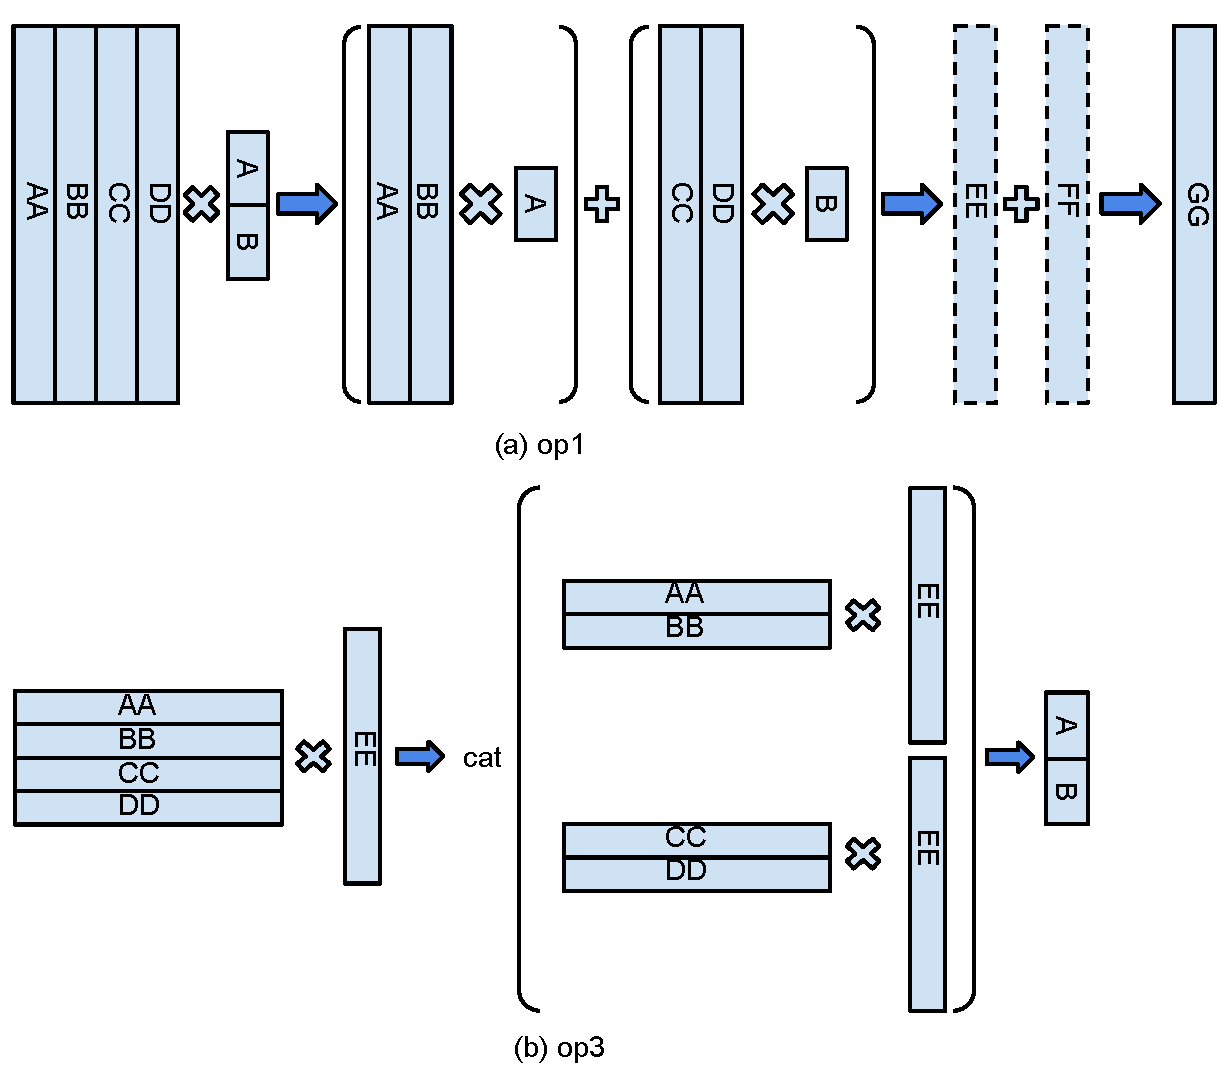
\includegraphics[scale=0.4]{./mat_group.pdf}
\vspace{-5pt}
\caption{}
\vspace{-5pt}
\label{fig:mat_group}
\end{figure}

The Anasazi eigensolvers frequently perform a matrix operation on many
tall-and-skinny matrices and the number of the matrices varies in each iteration.
The number of tall-and-skinny matrices can be as large as multiple hundred
in some eigensolvers when computing hundreds of eigenvalues.
Such an operation includes $op1$ and $op3$. If a thread has to read the data
of the same partition from all of the matrices, the amount of data in memory
can be very large. Because the matrices store elements in column-major order,
reading part of a partition results in many small reads and writes to SSDs.
In order to have large I/O to SSDs, we maintain the same partition size for
the matrices and break the large group of matrices into multiple small groups
when evaluating these operations on them.
hierarchically.

\dz{This approach actually can change the computation complexity of dense matrix
multiplication. I need to measure its impact on in-memory dense matrix
multiplication.}

When accessing a large group of matrices, we access matrix portions horizontally
before going vertically.
Optimization for a large group of dense matrices.

\subsubsection{Lazy evaluation} \label{sec:lazy_eval}
The Anasazi eigensolvers allows users to store the tall dense matrices and
implement the operations on the matrices themselves. Such flexibility allows
us to evaluate the dense matrix operations lazily \cite{Ching12} to avoid
materializing
every dense matrix, which reduces the amount of data read and written to SSDs.

Due to lazy evaluation, vectors in the subspace is immutable, so each operation
generates new vectors. Therefore, we group the vectors in the subspace into
dense matrices. The vectors in a dense matrix are updated together in the block
eigensolver. The number of vectors in a matrix is determined by the block
size of a block eigensolver. Once a dense matrix does not contain any vectors
referenced by the eigensolver, the dense matrix is garbage collected.

\begin{table}
	\begin{center}
		\small
		\begin{tabular}{|c|c|c|c|c|}
			\hline
			& operation & customized output \\
			\hline
			op9 & $AA \leftarrow conv\_layout(BB)$ & yes \\
			\hline
			op10 & $AA \leftarrow merge(BB, CC, ...)$ & yes \\
			\hline
			op11 & $[BB, CC, ...] \leftarrow split(AA)$ & yes \\
			\hline
		\end{tabular}
		\normalsize
	\end{center}
	\caption{Additional dense matrix operations required by FlashEigen.
		$XX$ represents a tall dense matrix.}
	\label{add_ops}
\end{table}

FlashEigen requires some additional operations to convert data layout
in dense matrices, as shown in Figure \ref{add_ops}.
We need an operator $conv\_layout(AA)$ to convert data layout
in the dense matrices. The eigensolvers require to access individual columns
of the tall matrices, so these dense matrices are stored in column major
to access them efficiently. However,
the sparse matrix dense matrix multiplication described in section \ref{spmm}
requires the dense matrix stored in row major to increase data locality.
Therefore, we store the dense matrices in column major by default. Only
when the dense matrices are passed to SpMM, they are converted to row major.

To enable lazy evaluation, we define a special matrix to represent the output
matrix from a matrix operation. Such a matrix does not store the data of
an operation result. Instead, it stores the computation and the reference to
the input matrices. We refer to these dense matrices as \textit{virtual matrices}.
Most matrix operations in Table \ref{ops} output \textit{virtual matrices},
as long as the output matrices are tall dense matrices. Only \textit{op3}
and \textit{op6} cannot be virtualized because they output small matrices and
small vectors.

With \textit{virtual matrices}, we construct a directed acyclic graph (DAG)
at runtime to represent computation in the eigensolvers. In the DAG, we store
all scalar variables and small matrices as part of computation.
Figure \ref{comp_seq} shows an example of a sequence of dense matrix operations
performed in the eigensolvers. Figure
\ref{dag} visualizes the sequence of computation, which forms a directed acyclic
graph (DAG). Inside this DAG, we do not need to perform any computation other
than the last one.

All matrices in the DAG need to be immutable so that \textit{virtual matrices}
can generate the same result any time when they are materialized. However,
the Anasazi eigensolvers originally reuse the existing matrices to store
the results of matrix operations as shown in Figure \ref{comp_seq}. Therefore,
our implementation of the matrix operations always generates new matrices and
the \textit{Anasazi matrices} only store pointers to matrix data. This approach
is equivalent to renaming variables used by compilers.

\textit{op7} and \textit{op8} access individual columns and have to be incorporated
with the lazy evaluation. The eigensolvers usually access only one column at a time
from a dense matrix. When accessing a single column, we materialize the virtual
matrix in column major if the underlying matrix is a \textit{virtual matrix}.
Because all matrices are immutable, setting a column in a matrix needs to
copy the original matrix and set the particular column. Instead of physically
generating the matrix, we create a virtual matrix that merge the original matrix
with the column.

\begin{figure}
\begin{minted}[mathescape,
		fontsize=\scriptsize,
		frame=single,
]{r}
# MV0, MV1, MV2, MV3, MV4 are tall dense matrices.
# B1, B2, B3, B4 are small dense matrices.
# MV1 is the result of sparse matrix dense matrix
# multiplication.
MV0 <- rand_init
MV1 <- SpMM
MV2 <- 1 * MV0 * B1 + 0 * MV2
MV2 <- 1 * MV2 * B2 + 0 * MV2
MV3 <- 1 * MV1 * B3 + 0 * MV1
MV1 <- -1 * MV2 * B4 + MV3
MV4 <- MV1 * diag(vec)
B <- t(MV4) * MV4
\end{minted}
\vspace{-5pt}
\caption{A small sequence of dense matrix operations typically performed by
the Anasazi eigensolvers.}
\label{comp_seq}
\end{figure}

\begin{figure}
\centering
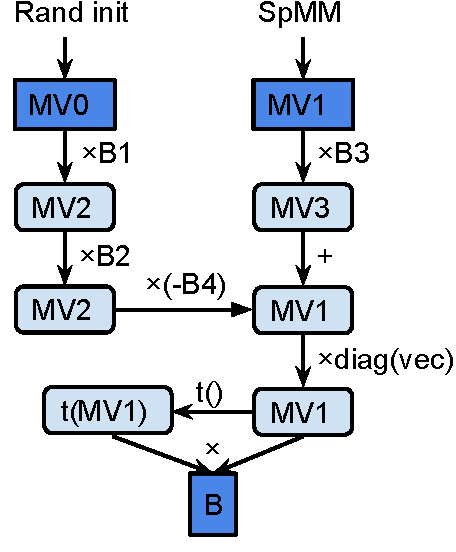
\includegraphics[scale=0.5]{./dag.pdf}
\vspace{-5pt}
\caption{A directed acyclic graph represents the sequence of matrix operations
shown in Figure \ref{comp_seq}. Each rounded rectangular node indicates
a virtual matrix and each rectangular node indicates a materialized matrix.}
\vspace{-5pt}
\label{dag}
\end{figure}

%vmat-7 = 1 * mem_mat-0(4039,4) * mem_mat-6(4,4)
%vmat-22 = 1 * vmat-7 * mem_mat-21(4,4)
%vmat-24 = 1 * mem_mat-10(4039,4) * mem_mat-23(4,4)
%vmat-26 = -1 * vmat-22 * mem_mat-25(4,4) + 1 * vmat-24
%vmat-29 = vmat-26* vec
%vmat-29(vmat-26(-1 * vmat-22(1 * vmat-7(1 * mem_mat-0(4039,4) * mem_mat-6(4,4)) * mem_mat-21(4,4)) * mem_mat-25(4,4) + 1 * vmat-24(1 * mem_mat-10(4039,4) * mem_mat-23(4,4)))* vec)

\subsubsection{Materialize \textit{virtual matrices}}
The eigensolvers need to materialize \textit{virtual matrices} whenever
encountering \textit{op3} and \textit{op6} because the output of these two
operations is stored in Anasazi's native matrices and vectors. If the input
matrices of the operations are virtual matrices, we have to materialize them
first. This triggers matrix materialization recursively until we reach
the matrices that have been materialized. When materializing
a \textit{virtual matrix}, we materialize partitions of a matrix separately.
We discard the materialized partition of a matrix, once it is no longer needed,
to reduce the amount of data written to SSDs at the cost of extra computation.

We partition the virtual matrices horizontally in the same fashion as
the external-memory matrices, so that we can materialize each partion of
a virtual matrix independantly. 
When we materialize a partition of a matrix within a group of matrix
operations, we use a much smaller partition size than the external-memory
matrix to increase CPU cache hits. As such, we only need to read the input
matrix to CPU cache and the output of an operation is still in the CPU cache
when it is fed to the next operation as input.

As computation proceeds, the DAG grows and eventually becomes a very large graph.
In this large DAG, we would have to keep all materialized dense matrices on SSDs
and each matrix operation would involve in many dense matrices. Therefore, it
becomes prohibitively expensive in terms of space usage, computation and I/O
access if we do not trim the DAG. To trim the DAG, we materialize some of
the virtual matrices in the DAG. The current criteria is to materialize a virtual
matrix if the matrix depends on a certain number of materialized matrices.
We vary the threshold to trade off the amount of data read from SSDs and written
to SSDs. When the threshold is smaller, we only need to maintain a smaller DAG
in the cost of materializing more dense matrices on SSDs. By default, the number
is two. \dz{we should perform experiments to justify the default number.}

We materialize a matrix if it relies on more than two materialized matrices.
We also make sure all dense matrices in the basis are materialized.
\dz{It seems that we can save some multiplication. Why?}

\subsubsection{Data and computation sharing in the DAG}
When materializing matrices in the DAG, we materialize them recursively.
As a result, the matrices that are depended by multiple other virtual matrices
potentially have to be materialized multiple times. Thus, we buffer the
recently materialized partitions temporarily to save I/O and computation.
We buffer the materialized partitions in the local thread, so accessing them
doesn't incur any locking overhead.
This is feasible because all tall matrices are partitioned horizontally and .

\dz{Only buffer data in the matrix where data can be shared.}

When we buffer the recent portions, we need to give each matrix a data identifier
to identify its data, so we can recognize which portion of data can be reused.
For certain operations, even though a new matrix is created, the data inside
remains the same. A typical example is transpose. The identifier we give to
each matrix should identify the data inside a matrix instead of individual matrices,
so a transposed matrix and its original matrix should share the same identifier.

We only cache one portion of data from each matrix. This is enough for the current
computation model.

The entire portion in the EM matrix should be processed by a single thread in order
to have the cached data being reused.

\subsubsection{Caching}

We can cache the most recently materialized matrix in memory.
